%enemies.tex
Here a list of all enemies with a short description is given. Enemies information are obtained from: 
\begin{itemize}
	\item X1: \cite{wayback:X_resources},\cite{wiki:X1_enemies},
	\item X2: \cite{wayback:X2_resources},\cite{wiki:X2_enemies}
	\item X3: \cite{wayback:X3_resources},\cite{wiki:X3_enemies}
\end{itemize}
while all artworks come from \cite{book:MMX_Complete_art}. In some occasions artworks from the XDive game will also  be shown.

\section{Mini-Bosses}
\begin{itemize}
	\item \hypertarget{miniboss:Anglerge}{\textbf{Anglerge}}:
	\enemSpecs{64 ($\sim$0.15 seconds of Iframe, Boomerang Cutter, Rolling Shield and Sting Chameleon hit for 8 damage) }{4 (contact), 2 (snakes)}{Angler-type mechaniloids that work to cleaning the seabed floor, with a motion sensor attached to its "lantern" part.}
	\begin{figure}[htp]
		\centering
		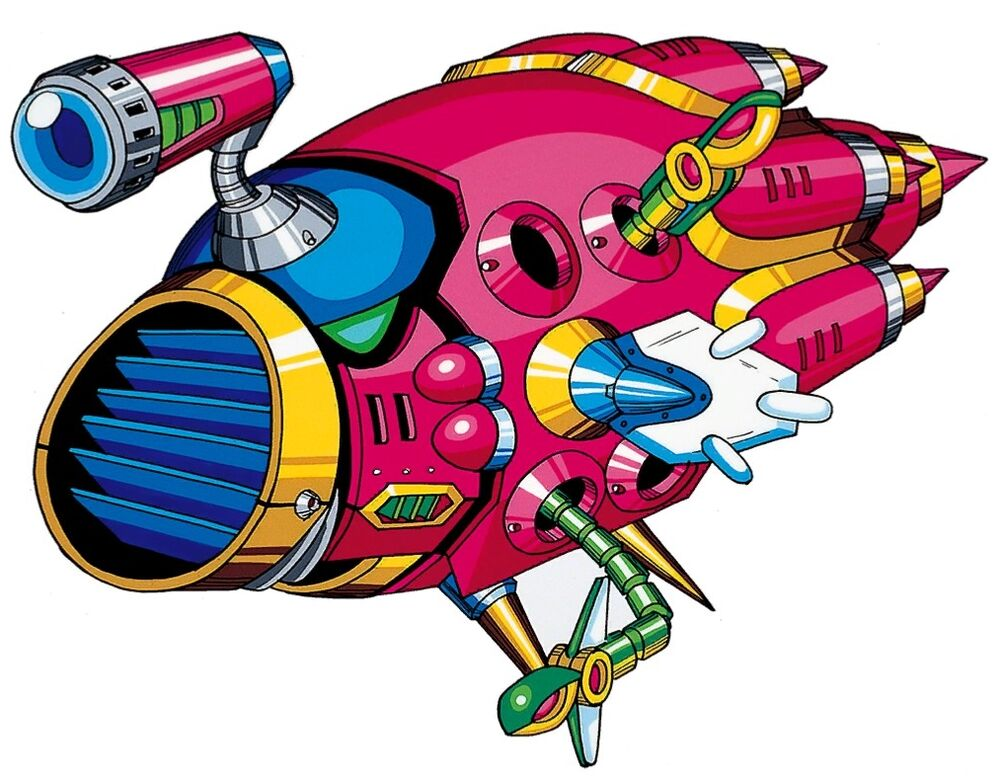
\includegraphics[height=3.5cm]{figures/X1/Enemies/Anglerge.jpg}
		\caption{Anglerge's artwork}
	\end{figure}
	
	\item \hypertarget{miniboss:Bee_Blader}{\textbf{Bee Blader}}:
	\enemSpecs{32 (No Iframes)}{4 (contact), 2 (missiles), 1 (machine gun), instant death if X is under it when killed}{A large bee-type helicopter which was created in order to carry \hyperlink{enem:Ball_De_Voux}{Ball de Voux}. It is equipped with a vulcan machine-gun and homing missiles. This mechaniloid has been created for guerrilla operations in forests and cities.}
	\begin{figure}[htp]
		\centering
		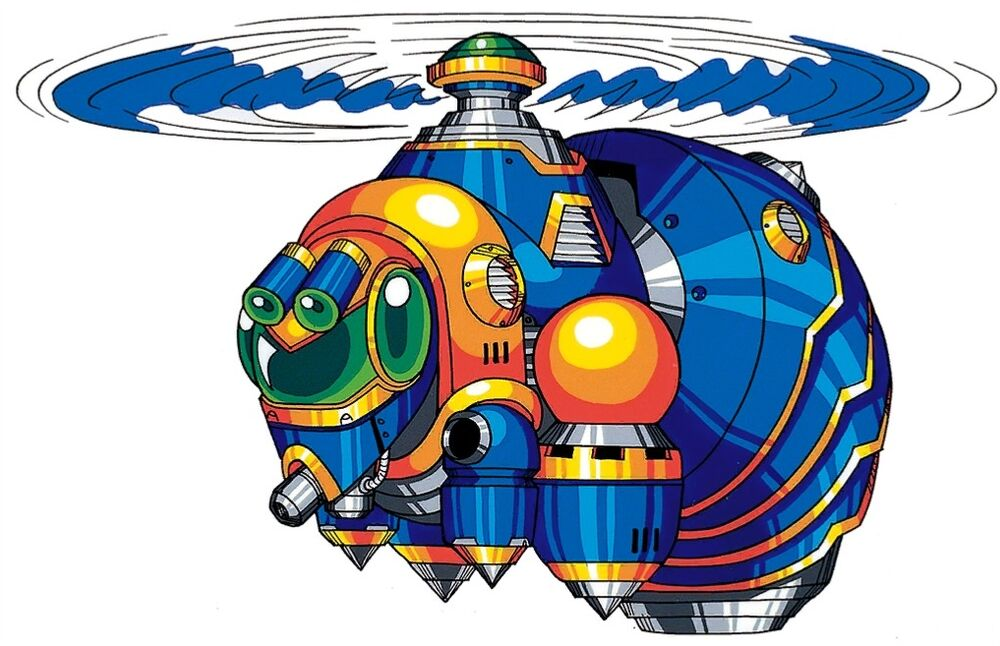
\includegraphics[height=3.5cm]{figures/X1/Enemies/BeeBlader.jpg}
		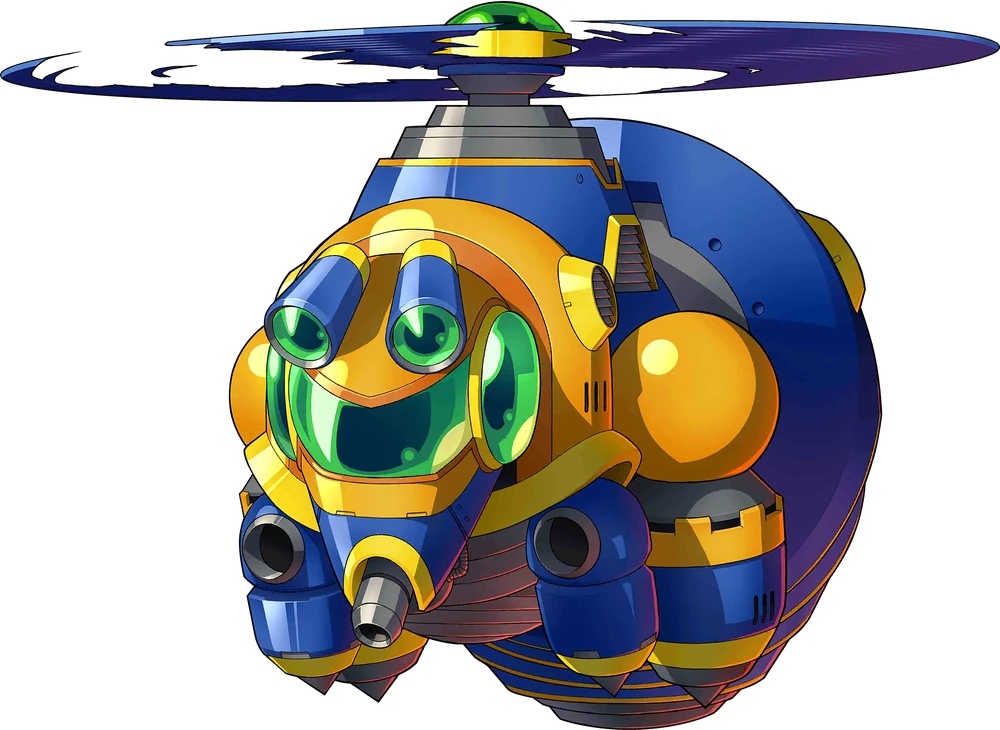
\includegraphics[height=3.5cm]{figures/X1/Enemies/BeeBlader_Dive.png}
		\caption{Bee Blader's artworks}
	\end{figure}
	
	\item \hypertarget{miniboss:Chop_Register}{\textbf{Chop Register}}:
	\enemSpecs{32 (weak only in the handle, a Giga Crush or a well-placed charged Sonic Slicer one shots it)}{2 (contact)}{Sigma Virus substantiated into sword form. Its patterns are based on Sigma's own saber skill.}
	\begin{figure}[htp]
		\centering
		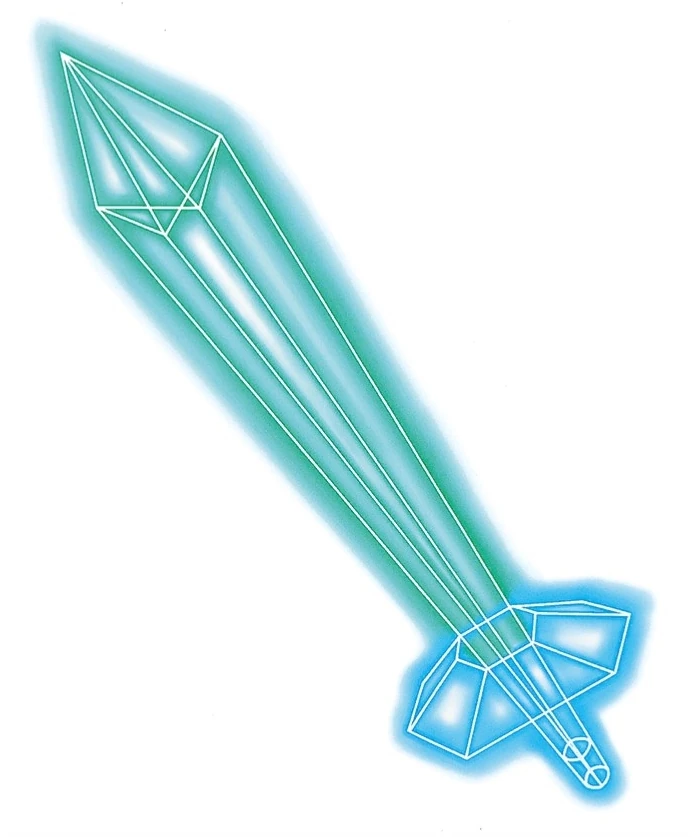
\includegraphics[height=3.5cm]{figures/X2/Enemies/ChopRegister.png}
		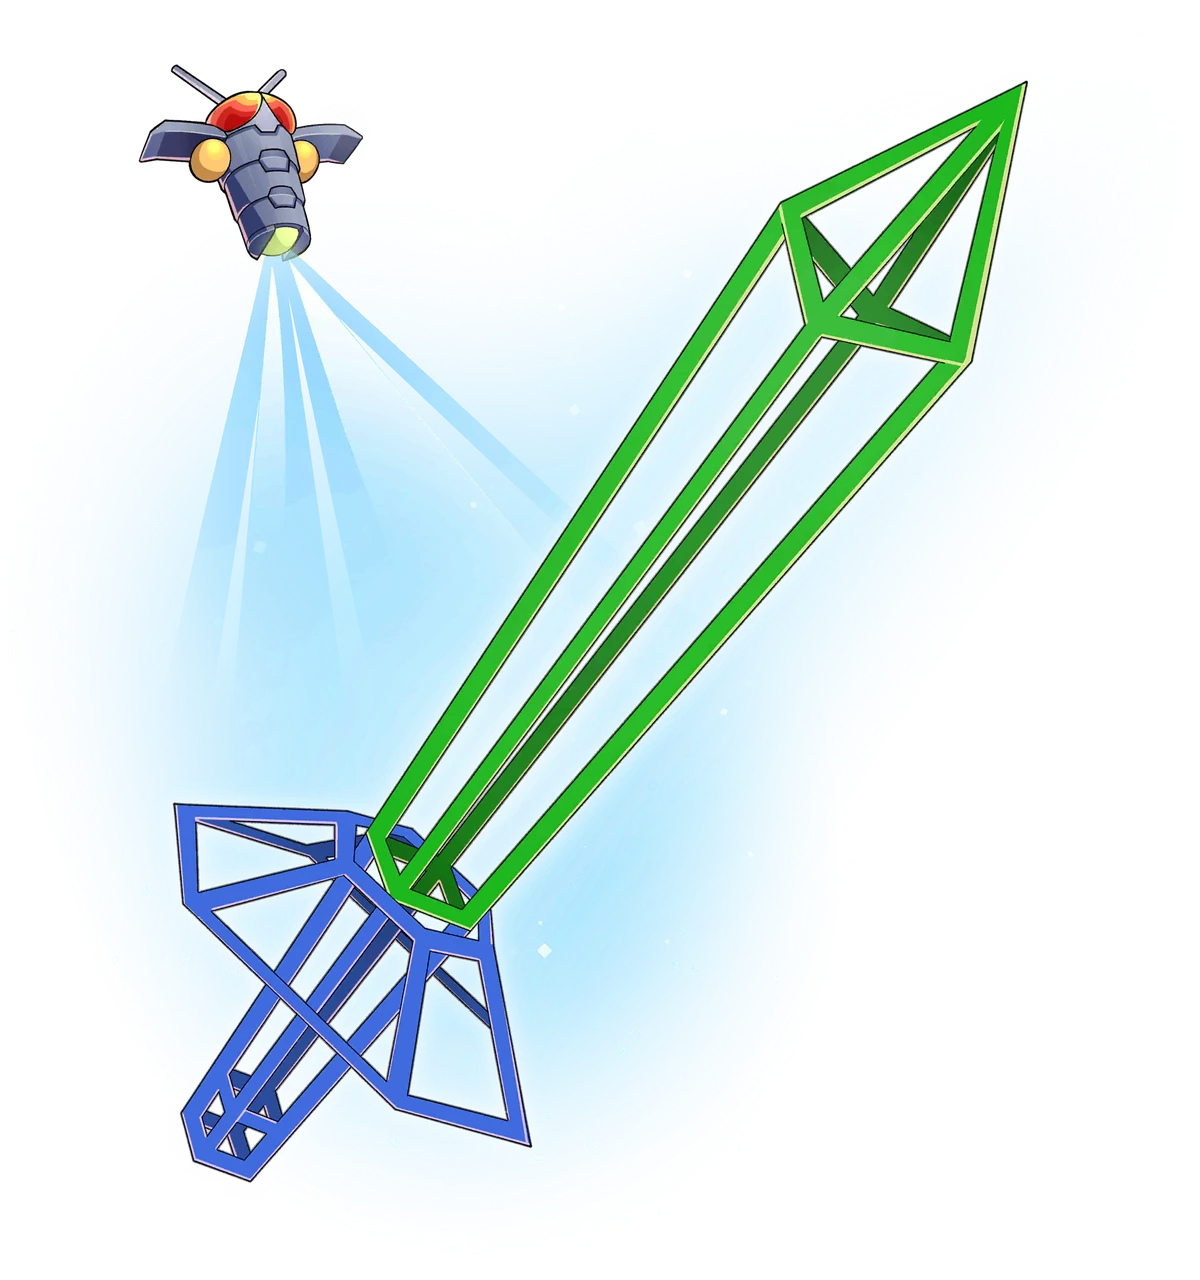
\includegraphics[height=3.5cm]{figures/X2/Enemies/ChopRegister_Dive.png}
		\caption{Chop Register's artworks }
	\end{figure}

	\item \hypertarget{miniboss:Cruiziler}{\textbf{Cruiziler}}: 
	\enemSpecs{64 (resist most weapons but no Iframes, a Storm Tornado is a guaranteed kill)}{3 (bombs)}{Whale mechaniloid who patrols the sea with its powerful weapon. Some kind of error caused it to lose its sea navigation systems, its attack circuits began running wild, and communications were lost. Its body is totally invincible, save for its core on top.}
	\begin{figure}[htp]
		\centering
		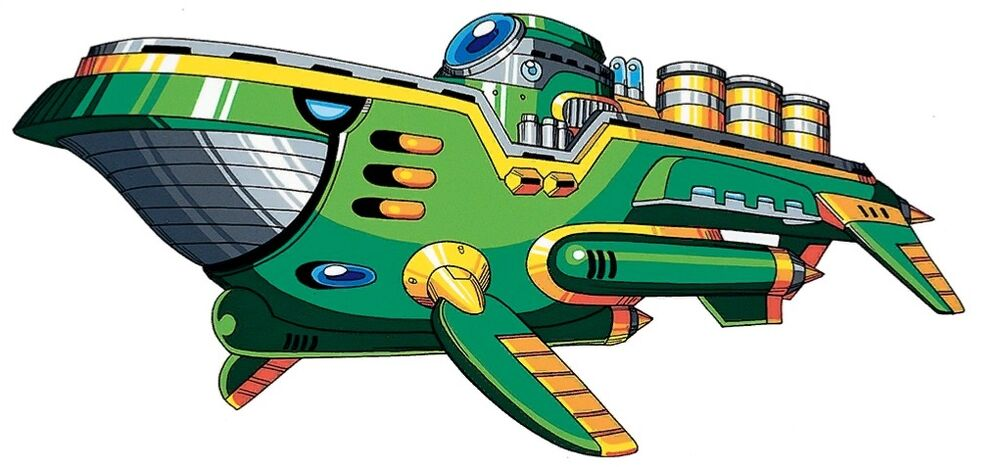
\includegraphics[height=3.5cm]{figures/X1/Enemies/Cruiziller.jpg}
		\caption{Cruiziller's artwork}
	\end{figure}
	
	\item \hypertarget{miniboss:Hell_Crusher}{\textbf{Hell Crusher}}:
	\enemSpecs{32 (no Iframes, a charged Triad Thunder instantly kills him)}{2 (contact), 2 (spikes), 3 (claw)}{A repliroid who, like Tunnel Rhino, participated in the mining of Energen Crystals. He can split its upper and lower body, for a powerful double attack.}
	\begin{figure}[htp]
		\centering
		
\includegraphics[height=3.5cm]{figures/X3/Enemies/hellcrusher.png}
		
\includegraphics[height=3.5cm]{figures/X3/Enemies/hellcrusher_dive.png}
		\caption{Hell Crusher's artworks}
	\end{figure}
	\item 
	\hypertarget{miniboss:Hotareeca}{\textbf{Hotareeca}}:
	\enemSpecs{32 (no Iframes)}{2 (contact), 2 (missiles), 3 (mines)}{A mechaniloid built to be a smaller version of Volt Kurageil. It is equipped with depth charges and homing missiles, but its tentacles can't seem to move together. Its low stamina makes it rather weak.}
		\begin{figure}[htp]
		\centering
		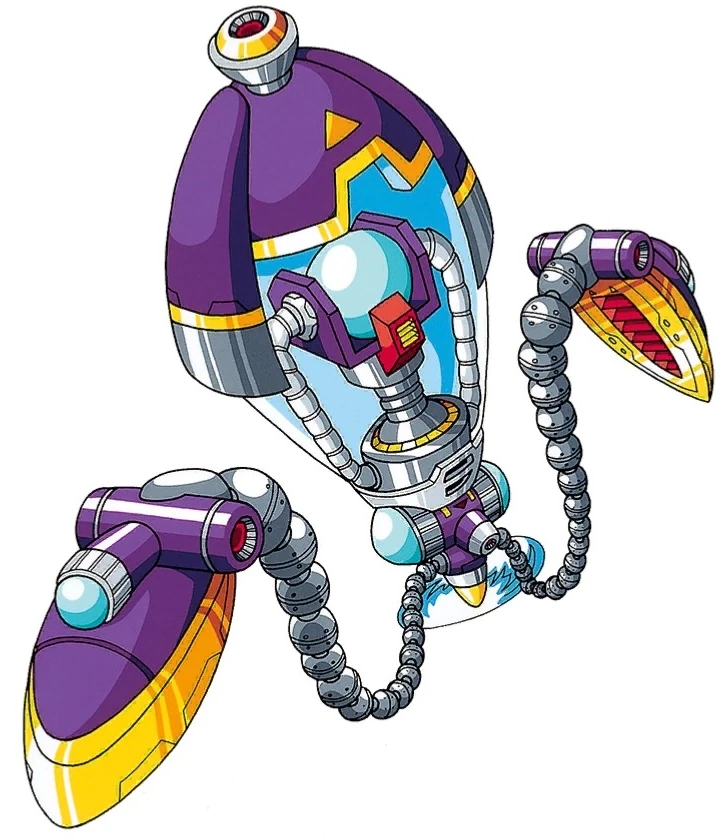
\includegraphics[height=3.5cm]{figures/X3/Enemies/hotareeca.png}
		\caption{Hotareeca's artworks}
	\end{figure}
	
	\item \hypertarget{miniboss:Mac}{\textbf{Mac}}:
	\enemSpecs{32 ($\sim$0.97 seconds of Iframes)}{2 (Parasitic Shot), 2 (Shot), 2 (Contact)}{Maverick Hunter soldier, who betrayed the hunters after being exposed to the Sigma virus.}
		\begin{figure}[htp]
		\centering
		
\includegraphics[height=3.5cm]{figures/X3/Enemies/mac.png}
		\caption{Mac's artworks}
	\end{figure}
	
	\item \hypertarget{miniboss:Magna_Quartz}{\textbf{Magna Quartz}}:
	\enemSpecs{20 ($\sim$0.97 seconds of Iframes, weak to silk shot)}{2 (contact with laser shooters), 2 (laser), 3 (contact with crystal)}{An unknown mechaniloid, embedded in a giant crystal. Attacks using 2 invincible support mechas, which fire reflecting lasers. Its true form inside the crystal is its weakness.}
	\begin{figure}[htp]
		\centering
		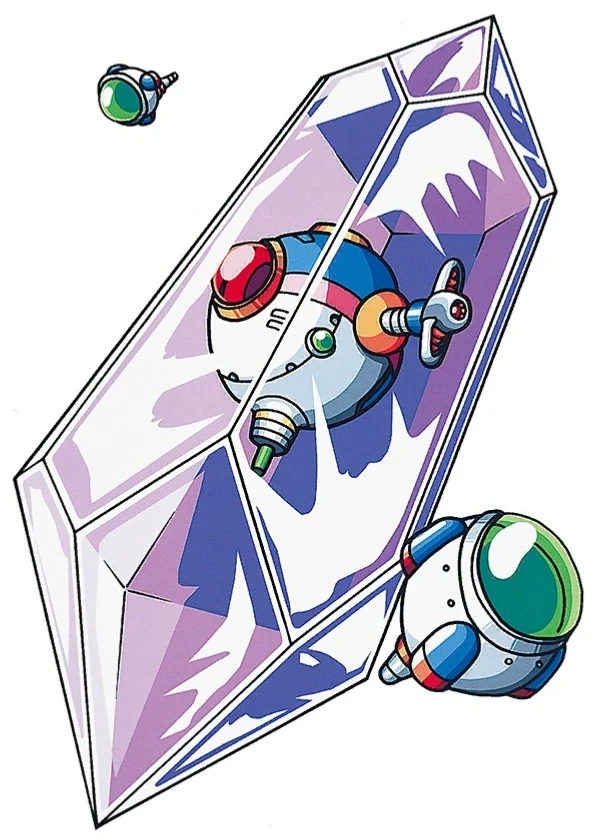
\includegraphics[height=3.5cm]{figures/X2/Enemies/MagnaQuartz.png}
		
\includegraphics[height=3.5cm]{figures/X2/Enemies/MagnaQuartz_Dive.png}
		\caption{Magna Quartz's artworks }
	\end{figure}
		
	\item \hypertarget{miniboss:Mole_Borer}{\textbf{Mole Borer}}:
	\enemSpecs{60 ($\sim$0.083 seconds of Iframes, the roller is invincible. Fire Wave deals 3 damage each 2 frames, making the best option from behind)}{Insta-kill (roller), 2 (contact)}{Mechanioid used to open up paths in mines, using a rotary roller to destroy rocks that obstruct its path. Its armoring can take a lot of damage, while the roller is completely invincible and can instantly kill X.}
	\begin{figure}[htp]
		\centering
		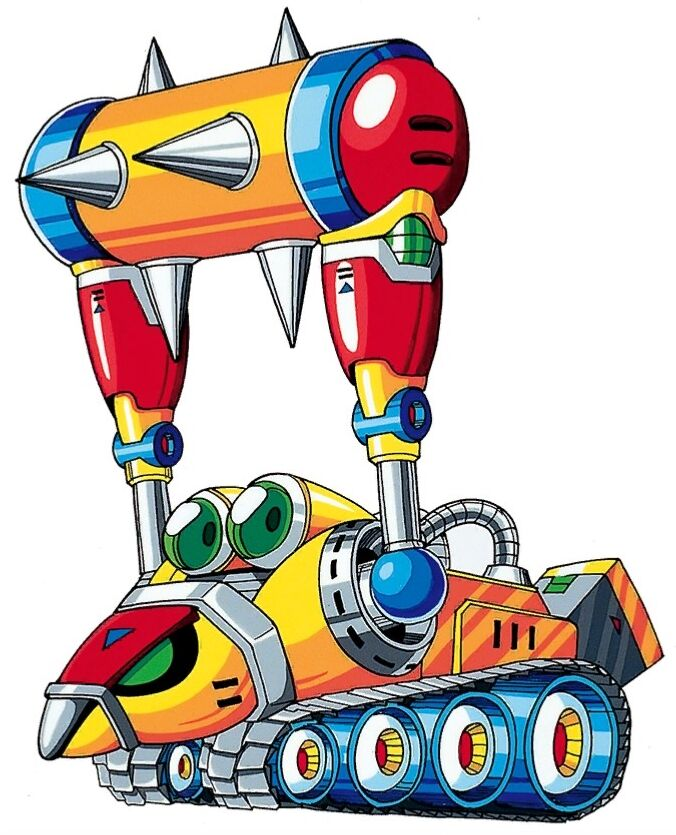
\includegraphics[height=3.5cm]{figures/X1/Enemies/MoleBorer.jpg}
		
\includegraphics[height=3.5cm]{figures/X1/Enemies/MoleBorer_Dive.png}
		\caption{Mole Borer's artworks}
	\end{figure}

	\item \hypertarget{miniboss:Mosquittus}{\textbf{Mosquittus}}:
	\enemSpecs{32 (Cross charge shot deals 18 damage, base Spinning Blade hits for 15 and charged Spinning Blade hist for 30 damage. Charged Tornado Fang kills him if it grabs X while holding it)}{0 (slime), 2 (acid pool),  4 per hit (drain), 4 (fire pillar, gas, acid), 8 (contact)}{It attaches itself to its victim, and drains their energy. It can also drain from the tanks below its room and change its attack power.}
	\begin{figure}[htp]
		\centering
		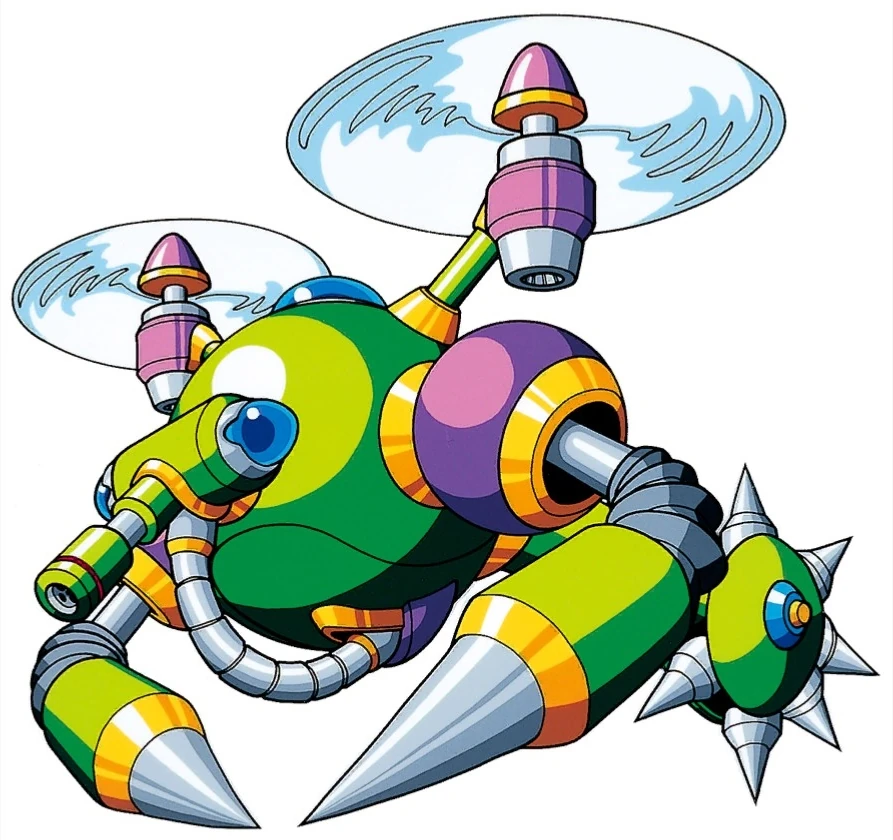
\includegraphics[height=3.5cm]{figures/X3/Enemies/mosquitus.png}
		\caption{Mosquittus's artwork}
	\end{figure}

	\item \hypertarget{miniboss:Old_robot}{\textbf{Old Robot}}:
	\enemSpecs{10, weak to Silk Shot, Magnet Mine and Spin Wheel. A well placed charged Spin Wheel or Silk shot one-shots it. Resurrect if the \hyperlink{miniboss:Pararoid_S-38}{Pararoid S-38} is not defeated quickly}{2 (scrap shot), 2 (contact)}{Combat robot used in wars of the past. Heavily armored, attacks were once useless on this invincible robot, but with the end of the wars, it was turned to scrap.}
	\begin{figure}[htp]
		\centering
		
\includegraphics[height=4cm]{figures/X2/Enemies/OldRobot.png}
		
\includegraphics[height=4cm]{figures/X2/Enemies/OldRobot_Dive.png}		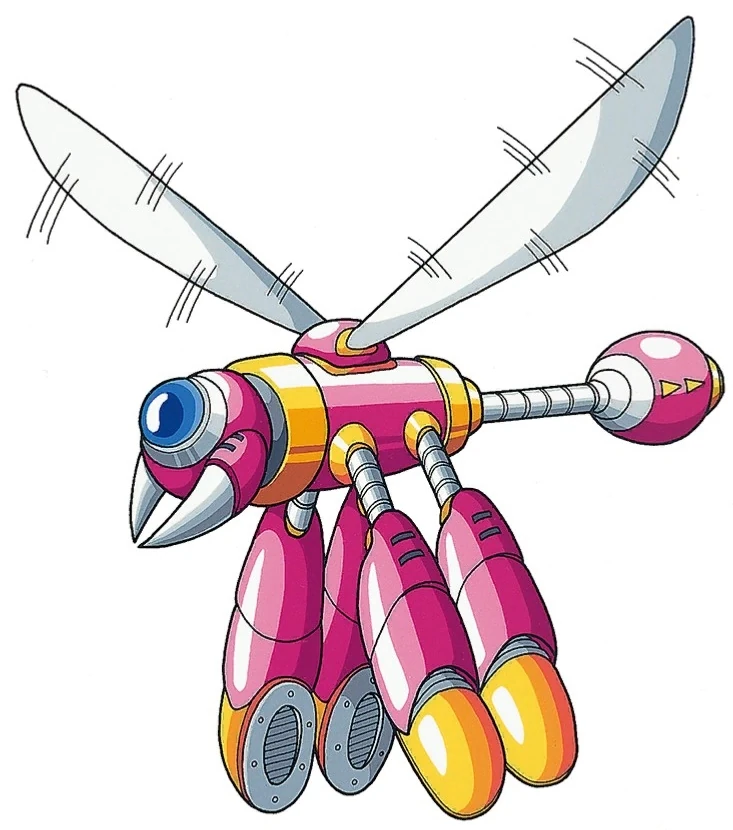
\includegraphics[height=2cm]{figures/X2/Enemies/PararoidS38.png}
		\caption{Old Robot and Pararoid S-38's artwork}
	\end{figure}
	
	\item \hypertarget{miniboss:Pararoid_S-38}{\textbf{Pararoid S-38}}:
	\enemSpecs{12, instantly killed by Sonic Slicer, Speed Burner and Giga Crush}{2 (contact)}{Next generation \hyperlink{enem:Pararoid_V-1}{Paraloid} prototype. Equipped with the ability of flight and improved durability, it posses the \hyperlink{miniboss:Old_robot}{Old Robot}, controlling it completely.}
	
	\item \hypertarget{miniboss:Raider_Killer}{\textbf{Raider Killer}}:
	\enemSpecs{32 in all forms ($\sim$0.5 seconds of Iframe, Speed Burner deal 3-6 damages)}{2 (hand cannon), 3 (scatter shots), 4 (contact), 2 (shield)}{Extra-large sized private intruder (Raider) repulsion mechaniloid. When it searches an enemy with its radar, it scans the enemy's combat patterns as well. When the radar discovers an enemy, Raider Killer's form is strengthened with a blue energy, and it enters a violent rage.}
	\begin{figure}[htp]
		\centering
		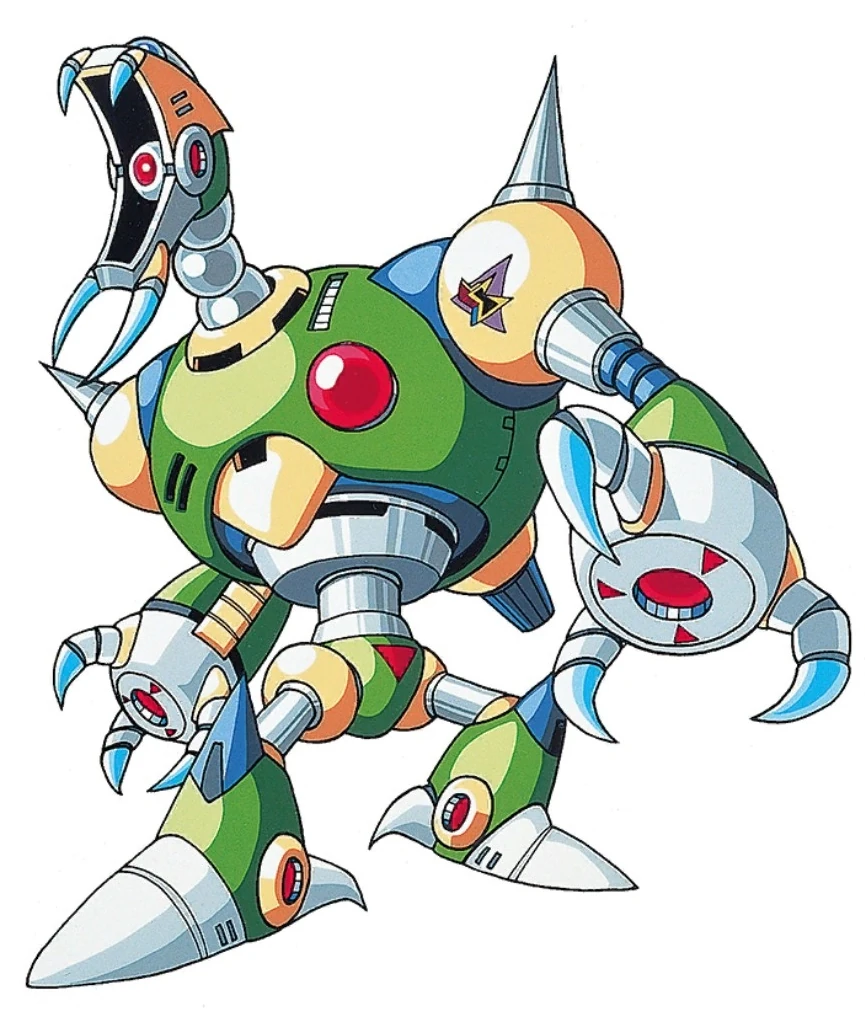
\includegraphics[height=3.5cm]{figures/X2/Enemies/RaiderKiller.png}
		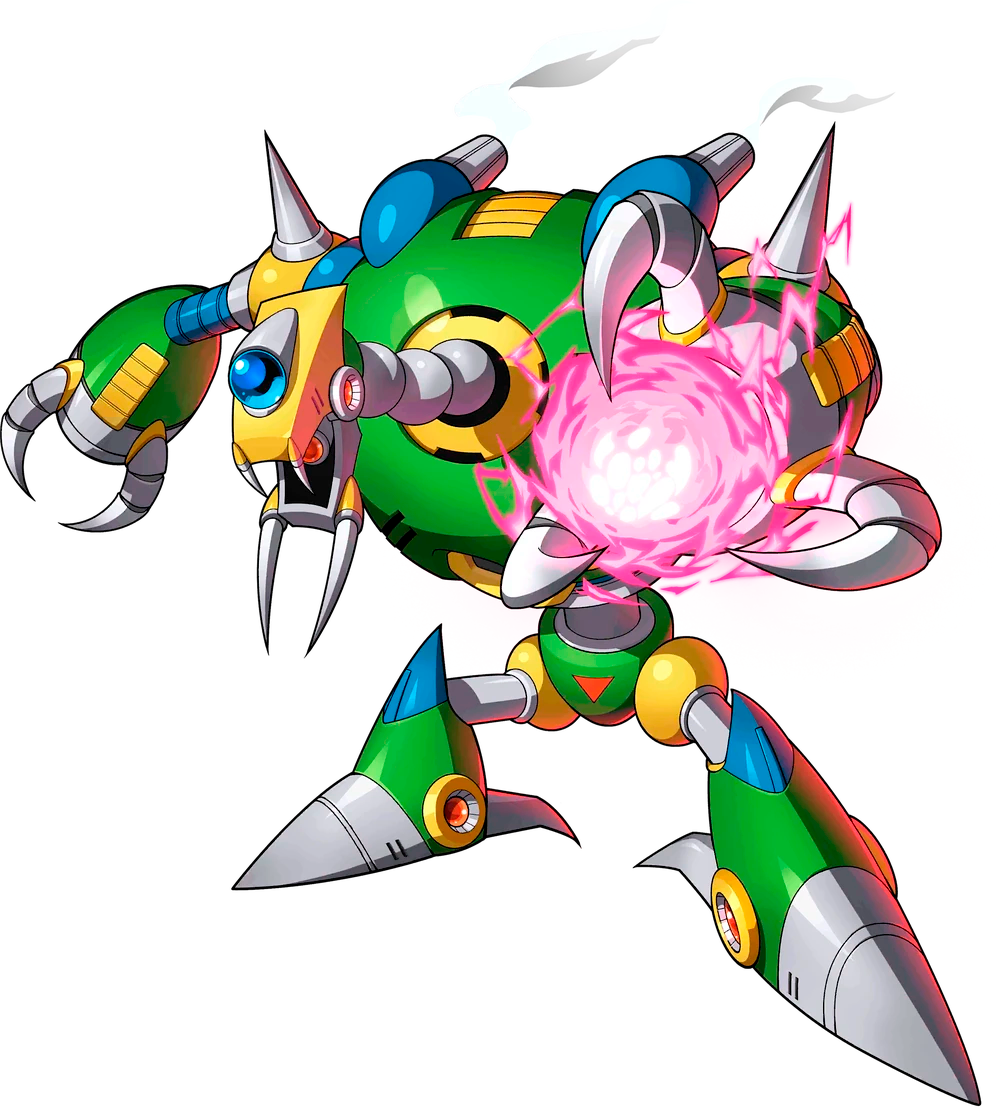
\includegraphics[height=3.5cm]{figures/X2/Enemies/RaiderKiller_Dive.png}
		\caption{Raider Killer's artworks}
	\end{figure}

	\item \hypertarget{miniboss:REX}{\textbf{REX-2000}}:
	\enemSpecs{32 ($\sim$0.97 seconds of invincibility frames per hit)}{2 (bullets), 4 (missiles), 8 (contact)}{Mechaniloid tank developed as an improved D-REX. The ability to walk has been added but, like the ride armors, an operator is necessary.}
	\begin{figure}[htp]
		\centering
		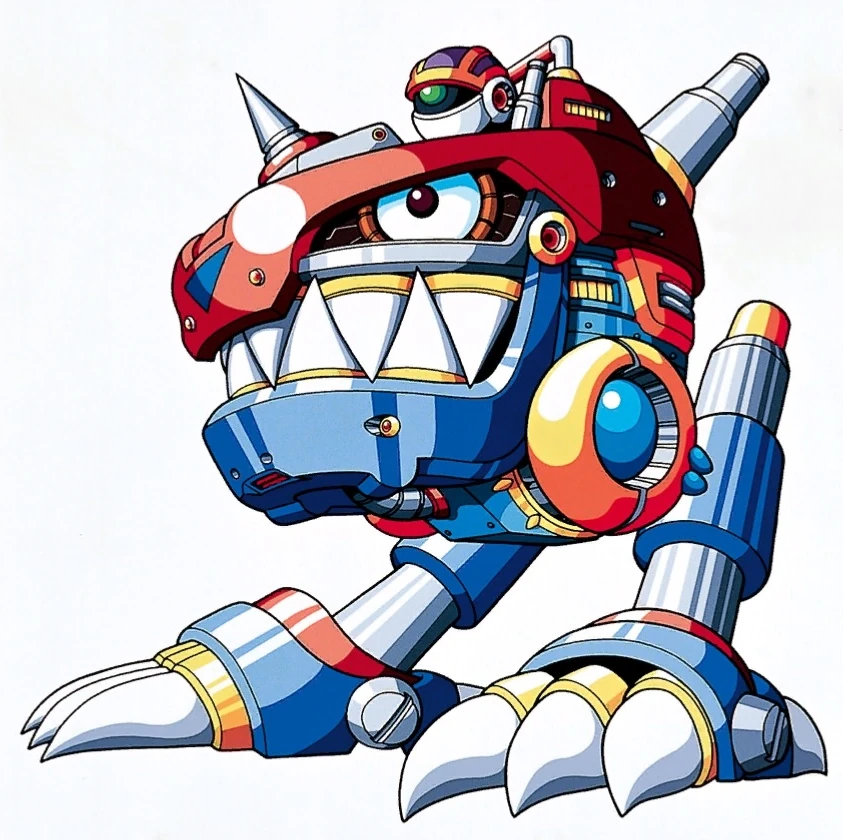
\includegraphics[height=3.5cm]{figures/X3/Enemies/rex2000.png}
		
\includegraphics[height=3.5cm]{figures/X3/Enemies/rex200_dive.png}
		\caption{REX-2000's artworks}
	\end{figure}	
			
	\item \hypertarget{miniboss:RT-55J}{\textbf{RT-55J}}: 
	\enemSpecs{64 ($\sim$0.5 second of Iframes, resist most weapons. Boomerang Cutter deals 3 damage instead of 2)}{2 (contact), 2 (arm)}{In times of peace, it was a professional robot sumo wrestler and a popular Yokozuna in the "Robot Grand Sumo Tournament". Moved in the forest, it now guards X's  Chest Parts. Its certain kill technique, the "Kagizume Beam Hand," strikes and tosses its opponents but only if it is in his claw's reach range. Otherwise he'll just jump at it to close the gap.} 
	\begin{figure}[htp]
		\centering
		
\includegraphics[height=3.5cm]{figures/X1/Enemies/RT-55J.jpg}
		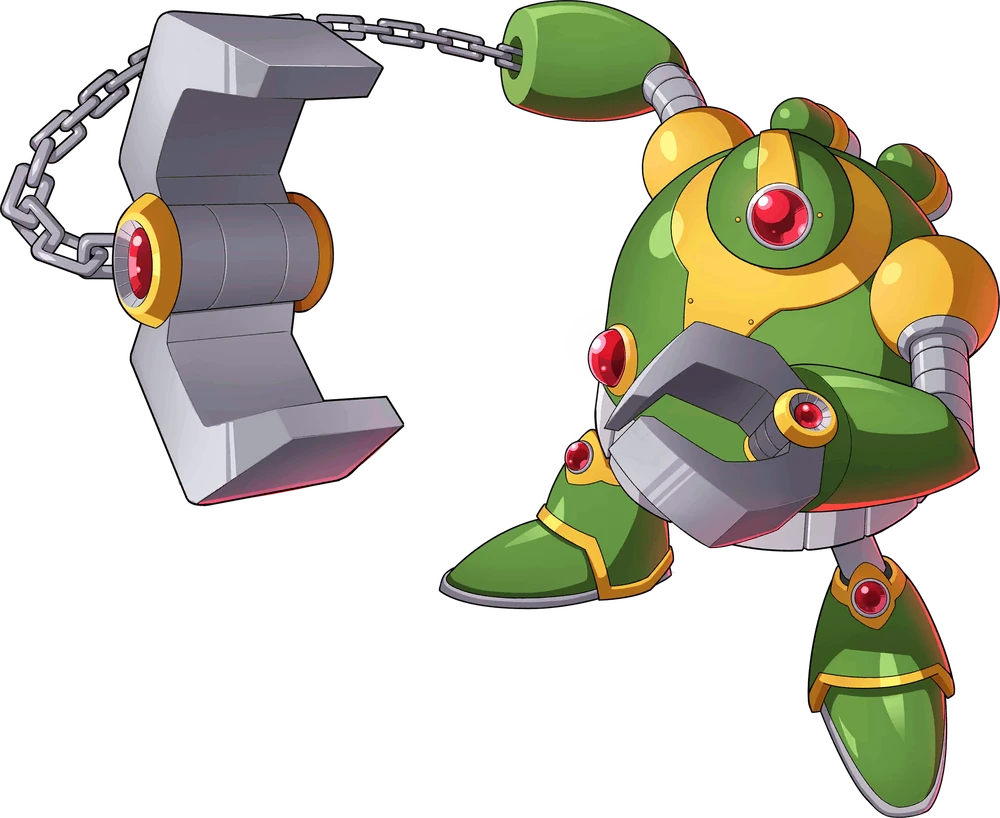
\includegraphics[height=3.5cm]{figures/X1/Enemies/RT55J_Dive.png}
		\caption{RT-55J's artwork}
	\end{figure}
	
	\item \hypertarget{miniboss:Sea_Canthller}{\textbf{Sea Canthller}}:
	\enemSpecs{40 (caudal fin), 24 (anal fin), 14 (breast), 10 (pectoral fin), 10 (front dorsal fin), 8 (lower dorsal fin), 4 (eyes), 4 (mouth)~\cite{wiki:Sea_Canthller} }{1 (laser), 3 (contact), 4 (mines)}{Originally, a deep sea working vessel designed as a mother ship for servicing and replenishing the \hyperlink{enem:Jelly_Seeker}{Jelly Seekers}. Now it has been remodeled as a transport unit that carries weapons to protect its cargo.}
	\begin{figure}[htp]%
		\centering
		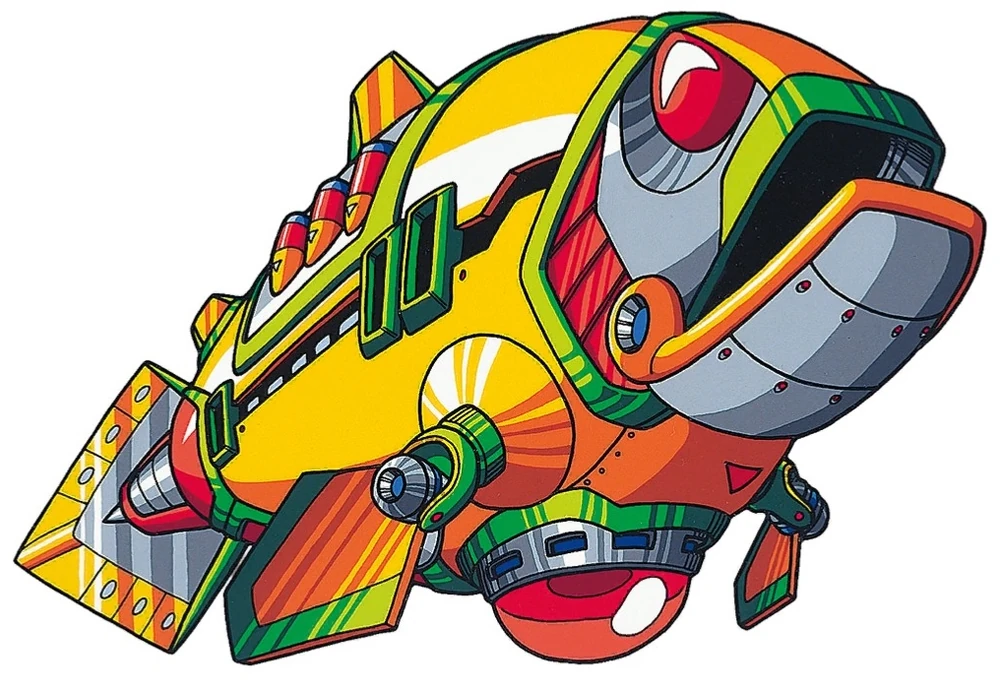
\includegraphics[height=3cm]{figures/X2/Enemies/SeaCanthller.png}
		\caption{Sea Canthller's artwork}
	\end{figure}
	
	\item \hypertarget{miniboss:Shurikein}{\textbf{Shurikein}}:
	\enemSpecs{18 ($\sim$0.97 seconds worth of invincibility frames)}{3 (contact)}{A substantiation of the Sigma Virus. It moves and attacks at random from 
	3 patterns. Its name comes from "shikein" and "shuriken". The flying mechaniloid that generates it is called Genjibo.}
	\begin{figure}[htp]%
		\centering
		
\includegraphics[height=3.5cm]{figures/X3/Enemies/shurikein.png}
		
\includegraphics[height=3.5cm]{figures/X3/Enemies/shurikein_dive.png}
		\caption{Shurikein (and Genjibo)'s  artwork}
	\end{figure}
	\item \hypertarget{miniboss:Thunder_Slimer}{\textbf{Thunder Slimer}}: 
	\enemSpecs{48 ($\sim$0.116 seconds of Iframes, Storm Tornado hits for 9-10 damage)}{5 (contact), 4 (thunders)}{Thunder Slimer was born from a single question: \textit{``How large can a single cell become?''} This monster was born from said experiment. Its body is over three times as large as X, but it should require approximately 10 more years before it reaches full growth. It has settled in the power plant, where it absorbs electricity and uses it to perform electric attacks against X.}
	\begin{figure}[htp]
		\centering
		
\includegraphics[height=3.5cm]{figures/X1/Enemies/ThunderSlimer.jpg}
		\caption{Thunder Slimer's artwork}
	\end{figure}
	
	\item \hypertarget{miniboss:Utuboros}{\textbf{Utuboros}}: 
	\enemSpecs{72, (no Iframes, Boomerang Cutter hits for 3 damage instead of 2 and Storm Tornado kills it in a single shot. Its body is invincible and can work as a platform, only the head and tail are vulnerable)}{4 (contact)}{Serpent-type mechaniloid made to explore the ocean floor. Thanks to its flexible body it can zig-zag into difficult underwater areas, and burrow underground.}
	\begin{figure}[htp]
		\centering
		
\includegraphics[height=3.5cm]{figures/X1/Enemies/Utuboros.jpg}
		\caption{Utuboros's artwork}
	\end{figure}
	
	\item \hypertarget{miniboss:Worm_seeker-r}{\textbf{Worm Seeker-R}}:: 
	\enemSpecs{64 (no Iframes, mines have 10 hp each)}{2 (mines), 4 (contact)}{Guardian from deep beneath Safari Park. It emerges, scatters 2 bombs, and dives back into the earth.}
	\begin{figure}[htp]
		\centering
		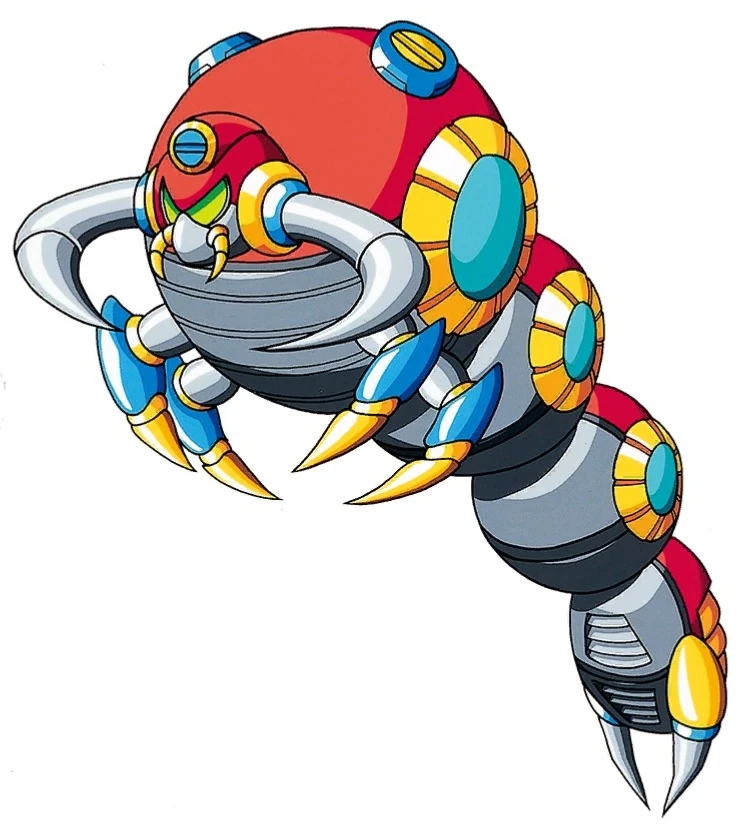
\includegraphics[height=3.5cm]{figures/X3/Enemies/wormseekerr.png}
		\caption{Worm Seeker-R's artwork}
	\end{figure}
\end{itemize}

%%%%%%%%%%%%%%%%%%%%%%%%%%%%%%%%%%%%%%%%%%%%%%%%%%%%%%%%%%%%%%%%%%%%%%%%%%%%%
%%%%%%%%%%%%%%%%%%%%%%%%%%%%%%%%%%%%%%%%%%%%%%%%%%%%%%%%%%%%%%%%%%%%%%%%%%%
%%%%%%%%%%%%%%%%%%%%%%%%%%%%%%%%%%%%%%%%%%%%%%%%%%%%%%%%%%%%%%%%%%%
\section{Minor enemies}
\begin{itemize}
		
	\item[{
\includegraphics[height=30px]{figures/X2/Enemies/sprite_aclanda.png}}] \hypertarget{enem:Aclanda}{\textbf{Aclanda}}:
	\enemSpecs{16, weak to Silk Shot, Spin Wheel and Magent Mine}{2 (grenades), 3 (laser), 4 (contact)}{Immobile artillery shaped like a scorpion, built by the X-Hunters to intercept the Maverick Hunters.}
	
	\item[{
\includegraphics{figures/X1/Enemies/sprite_amenhopper.png}}] \hypertarget{enem:Amenhopper}{\textbf{Amenhopper}}: 
	\enemSpecs{2}{1 (bombs), 2 (contact)}{Originally designed for farm work, it was used to sow fertilizer 
		across the land. Now, it's been remodeled into a bomb-dropping
		battle type mechaniloid.}

	
	\item[ {
\includegraphics[height=20px]{figures/X1/Enemies/sprite_armor_soldier.png}}] \hypertarget{enem:Armor_Soldier}{\textbf{Armor Soldier}}: 
	\enemSpecs{3 (on foot), 16 (Ride Armor)}{2 (contact, on foot), 3(contact-Armor)}{Lowest class of soldier reploids, used in military affairs. Riding in their Ride Armor, they do destruction work under Sigma's orders.}
	
	\item[{
\includegraphics[height=20px]{figures/X3/Enemies/Atareeter.png}}] \hypertarget{enem:Atareeter}{\textbf{Atareeter}}:
	\enemSpecs{10, weak to Parasitic Bomb}{2 (spiked trail), 8 (contact)}{Mechaniloid that uses its powerful teeth to shave the terrain into dangerous spike pits.} 
	
	\item[{
\includegraphics[width=30px]{figures/X1/Enemies/sprite_axemax.png}}] \hypertarget{enem:Axe_Max}{\textbf{Axe Max}}:
	\enemSpecs{8}{3 (contact), 2(flying log)}{Woodcutter reploid from the forest, remodeled for brutality. Swinging his large axe, he attacks by sending the chopped wood flying.}
	
	\item[{
\includegraphics[height=20px]{figures/X1/Enemies/sprite_balldevoux.png}}] \hypertarget{enem:Ball_De_Voux}{\textbf{Ball De Voux}}:
	\enemSpecs{2}{1 (contact)}{Equipped with 2 soft-treading feet, this mechaniloid can move over any topography.
		Inside the sphere there is a camera and a sensor which can even see in the dark.}
	
	\item[{
\includegraphics[height=30px]{figures/X2/Enemies/sprite_barwayings.png}}] \hypertarget{enem:Bar_Waying}{\textbf{Bar Waying}}:
	\enemSpecs{9, weak to Silk Shot, Spin Wheel and Magnet Mine}{2 (crush)}{This mechaniloid was developed as a shutter for disaster prevention. Extending its body, it attempts to block the path.}

	
	\item[{
\includegraphics[height=30px]{figures/X2/Enemies/sprite_BariteLastar.png}}] \hypertarget{enem:Barite_Lastar}{\textbf{Barite Lastar}}:
	\enemSpecs{2, weak to Silk Shot, Spin Wheel and Magnet Mine}{2 (laser), 2 (contact)}{Mechaniloid built for protecting military bases. It moves by attaching itself to a wall and can absorb enemy fire.}
	
	\item[{
\includegraphics[height=30px]{figures/X2/Enemies/sprite_BarrierAttacker.png}}] \hypertarget{enem:Barrier_Attacker}{\textbf{Barrier Attacker}}:
	\enemSpecs{2(must be hit behind the shield), weak to Strike Chain and Crystal Hunter}{2(contact)}{Loading work mechaniloid which equips a barrier for protection.}
	
	\item[{
\includegraphics{figures/X1/Enemies/sprite_battonbone.png}}] \hypertarget{enem:Batton_Bone}{\textbf{Batton Bone}}:
	\enemSpecs{1}{1 (contact)}{Bat mechaniloids with a taste for humans. They dwell in forests and caves.}
	
	\item[{
\includegraphics{figures/X1/Enemies/sprite_battonbone.png}}] \hypertarget{enem:Batton_Bone_type_G}{\textbf{Batton Bone type G}}:
	\enemSpecs{1}{1 (contact)}{Batton Bone like those of the previous production, upgraded with strengthened armor.}
	
	\item[{
\includegraphics[height=15px]{figures/X1/Enemies/sprite_battonm501.png}}]  \hypertarget{enem:Batton_M-501}{\textbf{Batton M-501}}: 
	\enemSpecs{2}{1 (contact)}{Bat type mechaniloid which the \hyperlink{enem:Batton_Bone}{Batton Bone} series is based on. It is a very unusual mechaniloid, made over 30 years ago.}
	
	\item[{
\includegraphics[height=30px]{figures/X2/Enemies/sprite_beetron.png}}] \hypertarget{enem:Beetron}{\textbf{Beetron}}:
	\enemSpecs{16, weak to Silk Shot, Spin Wheel and Magnet Mine}{4 (contact)}{Beetle type mechaniloid designed for work in the mines.}
	
	\item[{
\includegraphics[height=20px]{figures/X3/Enemies/bladeysprite.png}}] \hypertarget{enem:Blady}{\textbf{Blady}}:
	\enemSpecs{7, weak to Parasitic Bomb and Gravity Well}{2 (contact)}{Mechaniloid similar to \hyperlink{enem:Spiky}{Spiky}, it unleashes sharp blades and charges}
	
	
	\item[{
\includegraphics[height=30px]{figures/X2/Enemies/sprite_blecker.png}}] \hypertarget{enem:Blecker}{\textbf{Blecker}}:
	\enemSpecs{6, weak to Silk Shot, Spin Wheel and Magnet Mine}{2 (orbs), 2 (contact)}{Energy cannon which operates during an emergency. When not in operation, this mechaniroid is harmless.}
	
	\item[{
\includegraphics{figures/X1/Enemies/sprite_bombeen.png}}]\hypertarget{enem:Bomb_Been}{\textbf{Bomb Been}}:
	\enemSpecs{2}{2 (contact), 1 (bomb)}{Small bee-modeled helicopter used for land mines scattering. Able to infiltrate any area, it can set up land mines anywhere.}
	
	\item[{
\includegraphics[height=30px]{figures/X2/Enemies/sprite_CannonDriver.png}}] \hypertarget{enem:Cannon_Driver}{\textbf{Cannon Driver}}:
	\enemSpecs{14, weak to Silk Shot, Spin Wheel and Magnet Mine}{2 (contact), 4 (cannon)}{2-footed walker type interceptor mechaniloid. Powerful tank, it fires using two 200 mm cannons and enemy-seeking pursuit missiles.}
	
	
	
	\item[{
\includegraphics[height=20px]{figures/X3/Enemies/carryarmsprite.png}}] \hypertarget{enem:Carry_Arm}{\textbf{Carry Arm}}: 
	\enemSpecs{3, never appear if Gravity Beetle is defeated before Blast Hornet}{2 (contact)}{Conveyance robot used to help move supplies from the armory to the flying aircraft carrier. It has no offensive attacks.}

	\item[{
\includegraphics[height=20px]{figures/X3/Enemies/caterkillersprite.png}}] \hypertarget{enem:Caterkiller}{\textbf{Caterkiller}}:
	\enemSpecs{2, weak to Parasitic Bomb and Gravity Well}{2 (contact), 3 (electric spheres), 3 (contact-charged), 8 (charged electric spheres)}{Caterpillar-type mechaniloid which can move alongside walls. The range of its lightning shot is short, but it always returns to its body.}
	
	\item[{
\includegraphics[width=30px]{figures/X3/Enemies/Crablaster.png}}] \hypertarget{enem:Crablaster}{\textbf{Crablaster}}:
	\enemSpecs{4}{2 (contact), 3(projectiles), 3(barrier)}{Ambusher mechaniloid that moves by clinging to the ceiling or floor. When its artillery is broken, it creates a defensive barrier around itself.}
	
	\item[{\includegraphics[height=20px]{figures/X1/Enemies/sprite_cragman.png}}] \hypertarget{enem:Crag_Man} {\textbf{Crag Man}}:
	\enemSpecs{8}{2 (contact),2 (rock fall)}{Crag Men were made to clear rock debris during landslides. They work actively with the aerial mechaniloid \hyperlink{enem:Sky_Claw}{Sky Claw}.}
	
	\item[{\includegraphics[height=15px]{figures/X2/Enemies/sprite_CrashRoader.png}}] \hypertarget{enem:Crash_Roader}{\textbf{Crash Roader}}:
	\enemSpecs{3, weak to Strike Chain and Crystal Hunter}{2 (contact)}{Member of a gang rival of the \hyperlink{enem:Road_Attackers}{Road Attackers}. Once they start rolling, they won't turn until they hit a wall}
	
	\item[{\includegraphics[height=10px]{figures/X1/Enemies/sprite_creeper.png}}] \hypertarget{enem:Creeper} {\textbf{Creeper}}:
	\enemSpecs{1}{1 (contact)}{An insect-type mechaniloid. It's unknown what it was made for.	It is pecked out from the insides of trees by the \hyperlink{enem:Mad_Pecker}{Mad Pecker}.}
	
	\item[{\includegraphics[height=20px]{figures/X2/Enemies/sprite_CroakHopper.png}}] \hypertarget{enem:Croak_hopper}{\textbf{Croak Hopper}}:
	\enemSpecs{4, weak to Sonic Slicer, Speed Burner and Bubble Splash}{1 (shots), 3 (contact)}{Once the mascots of the Weather Control Center, were later remodeled by the X-Hunters for attack.}
	
	\item[{\includegraphics[height=20px]{figures/X1/Enemies/sprite_crusher.png}}] \hypertarget{enem:Crusher}{\textbf{Crusher}}:
	\enemSpecs{2}{4}{Construction mechaniloid used for knocking down buildings. It drops its steel-made weight to scrape down the highway.}
	
	\item[{\includegraphics[height=20px]{figures/X1/Enemies/sprite_diglabour.png}}] \hypertarget{enem:Dig_Labour}{\textbf{Dig Labour}}: 
	\enemSpecs{4}{2(pickaxe), 3(contact)}{The greatest pickaxe worker in the world. He is a diligent reploid who works in the robot factory.}
	
	\item[{\includegraphics[height=20px]{figures/X2/Enemies/sprite_DiskBoy08.png}}] \hypertarget{enem:Disk_Boy_08}{\textbf{Disk Boy 08}}:
	\enemSpecs{6, weak to Strike Chain and Crystal Hunter}{2 (disc), 2 (contact)}{Reploid player of the combat sport "Snapper Disk", model number 8.}
	
	\item[{\includegraphics[height=20px]{figures/X1/Enemies/sprite_dodgeblaster.png}}] \hypertarget{enem:Dodge_Blaster}{\textbf{Dodge Blaster}}: 
	\enemSpecs{3}{2 (contact), 2(shots)}{Latest model of mobile cannon with "self-defense function", which makes it possible to avoid energy attacks before they can even get near it.}
	
	\item[{\includegraphics[height=30px]{figures/X3/Enemies/drillwayingsprite.png}}] \hypertarget{enem:Drill_Waying}{\textbf{Drill Waying}}:
	\enemSpecs{5}{3 (contact)}{When an enemy gets near, it extends its drill-like body to block the path.}
	
	\item[{\includegraphics[height=20px]{figures/X3/Enemies/DrimoleW.png}}] \hypertarget{enem:Drimole-W}{\textbf{Drimole-W}}:
	\enemSpecs{6, leave two drill when destroyed}{1 (grenades), 2 (drills), 4(contact)}{Tank mechaniloid that shoots troublesome drill bullets that block attacks.}

	\item[{\includegraphics[height=20px]{figures/X3/Enemies/earthcommandersprite.png}}] \hypertarget{enem:Earth_Commander}{\textbf{Earth Commander}}L
	\enemSpecs{1 (body), 2 (ring), 4(propeller)}{2 (contact), 3(roller)}{Patrol mechaniloid which flies up and down or approaches in a ``U'' pattern.  If its propeller is destroyed, its body will land and try for a rolling ground attack.}
	
	\item[{\includegraphics[height=20px]{figures/X3/Enemies/escanail.png}}]
	 \hypertarget{enem:Escanail}{\textbf{Escanail}}:
	\enemSpecs{3 to destroy the shell}{2 (contact)}{Mechaniloid which lazily crawls up and down spiked walls. It is possible to ride it by breaking its shell.}
	
	
	\item[{\includegraphics[height=15px]{figures/X2/Enemies/sprite_Fishern.png}}] \hypertarget {enem:Fishern}{\textbf{Fishern}}:
	\enemSpecs{1}{1 (contact)}{Formerly a mechaniloid for feeding cultivated fish. After being remodeled, it breaks everything in sight.}
	
	\item[{\includegraphics[height=20px]{figures/X1/Enemies/sprite_flamer.png}}] \hypertarget{enem:Flamer}{\textbf{Flamer}}:
	\enemSpecs{6}{3 (contact), 2(fire)}{High-temperature, blaze-blowing, flamethrower machine. A remodeled airport fire extinguisher mechaniloid, turned into a weapon which tries to spread fires.}
	
	\item[{\includegraphics[height=30px]{figures/X1/Enemies/sprite_flammingle.png}}] \hypertarget{enem:Flammingle}{\textbf{Flammingle}}:
	\enemSpecs{8, 4 (saw)}{3 (contact), 2(blade)}{Flamingo-type mechaniloid taken from the robot zoo. It attacks by spinning its head and releasing the saw.}
	
	\item[{\includegraphics[height=30px]{figures/X3/Enemies/GansekiCarrierwebp.png}}] \hypertarget{enem:Ganseki_Carrier}{\textbf{Ganseki Carrier}}:
	\enemSpecs{4, weak to Parasitic Bomb and Gravity Well}{2 (missiles), 4(boulders and spiked balls), 4(contact)}{Mechaniloid made for heavy lifting, adapted for combat. It will try to drop a heavy boulder onto an enemy, then land on the ground to attack with missiles.}
	
	\item[{\includegraphics[height=30px]{figures/X2/Enemies/sprite_GarakutaRobot.png}}] \hypertarget{enem:Garakuta_Robot}{\textbf{Garakuta Robot}}:
	\enemSpecs{8 total, 2 (hat), 2(head), 4(body, can regenerate broken parts), Silk Shot instantly kill)}{1 (contact)}{Ghastly mechaniloid made from broken \hyperlink{enem:Metall_C-15}{Metall}, \hyperlink{enem:Dig_Labour}{Dig Labours}, \hyperlink{enem:Gulpfer}{Gulpfers} and \hyperlink{enem:Spiky}{Spikys}}.
	
	\item[{\includegraphics[height=20px]{figures/X1/Enemies/sprite_gulpfer.png}}] \hypertarget{enem:Gulpfer}{\textbf{Gulpfer}}:
	\enemSpecs{10}{2 (contact), 2-32 (eating)}{Once the ornamental mascot mechaniloid of a seaside Chaya teahouse, it escaped and was converted for catching ocean fish. It was originally based on an old children's toy.}
	
	\item[{\includegraphics[height=20px]{figures/X1/Enemies/sprite_gunvolt.png}}] \hypertarget{enem:Gun_Volt}{\textbf{Gun Volt}}:
	\enemSpecs{16}{3 (contact), 2(sparks), 2(missiles)}{Mechaniloid developed for military use. A tank made for terrestrial combat, it attacks with missiles and high voltage bullets.}
	
	\item[{\includegraphics[height=20px]{figures/X3/Enemies/HammaHamma.png}}] \hypertarget{enem:Hamma_Hamma}{\textbf{Hamma Hamma}}:
	\enemSpecs{11}{2 (mace), 3 (contact)}{Mechaniloid that swings 2 spiked iron balls at enemies. Its armor is very thick, but it's vulnerable to attacks from behind.}
	
	\item[{\includegraphics[height=30px]{figures/X2/Enemies/sprite_HangedReploid.png}}] \hypertarget{enem:Hanged_Reploid}{\textbf{Hanged Reploid}}:
	\enemSpecs{1(head), 3(Body), weak to Sonic Slicer, Speed Burner and Bubble Splash }{2 (fireballs), 2(contact)}{Pitiful reploid left in the scrap processing yards. Will attack and try to cling to anything that approaches.}
	
	\item[{\includegraphics[width=30px]{figures/X3/Enemies/hangerter.png}}] \hypertarget{enem:Hangerter}{\textbf{Hangerter}}:
	\enemSpecs{2}{No damage}{Mechaniloid which uses magnetic force to suspend objects in mid-air.} 
		
	\item[{\includegraphics[height=20px]{figures/X3/Enemies/headgunnercustomer.png}}] \hypertarget{enem:Head_Gunner_customer}{\textbf{Head Gunner customer}}:
	\enemSpecs{6, weak to Parasitic Bomb and Spinning Blade}{1 (projectiles), 6(contact)}{\hyperlink{enem:Head_Gunner}{Head Gunner} with cannons attached, as well as a stronger armor. Made from the parts produced in the weapons factory stage.}
	
	\item[{\includegraphics[height=20px]{figures/X3/Enemies/headgunnermasspro.png}}] \hypertarget{enem:Head_Gunner_masspro}{\textbf{Head Gunner masspro}}:\enemSpecs{4, weak to Parasitic Bomb and Spinning Blade}{1 (projectiles), 4 (contact)}{Basic model Head Gunner mechaniloid, equipped with 2 missile guns. It has legs attached, but cannot walk.}
	
	\item[{\includegraphics[height=20px]{figures/X3/Enemies/helitsprite.png}}] \hypertarget{enem:Helit}{\textbf{Helit}}:
	\enemSpecs{2, weak to Parasitic Bomb and Gravity Well}{2 (contact), 3 (missiles)}{Mechaniloid that flies through the sky and fires missiles. Its flight is hindered due to the weight of the missiles. }
	
	\item[{\includegraphics[height=20px]{figures/X1/Enemies/sprite_hoganmer.png}}] \hypertarget{enem:Hoganmer}{\textbf{Hoganmer}}:
	\enemSpecs{8}{3 (contact), 2(spike ball)}{Fighter in the future grappling show "Robot Coliseum." It blocks the attacks of enemies with its shield, and attacks	by swinging its iron ball and chain.}
	
	\item[{\includegraphics[height=20px]{figures/X1/Enemies/sprite_hotarion.png}}] \hypertarget{enem:Hotarion}{\textbf{Hotarion}}:
	\enemSpecs{1}{2 (contact)}{A mechaniloid for nighttime patrol, it was made to save the firefly appearance from extinction. Shining, it flies through the sky.}
	
	\item[{\includegraphics[height=20px]{figures/X3/Enemies/icedevoux.png}}] \hypertarget{enem:Ice_De_Voux}{\textbf{Ice De Voux}}:
	\enemSpecs{7 total, 3 (Ice shell), 4 (core), regenerates shell after some time}{2 (debris), 2 (contact-core), 6 (contact-shell)}{Icy variation of \hyperlink{enem:Ball_De_Voux}{Ball De Voux}. There is no walking function, but it can hover,	and call upon chunks of ice to protect its body.}
	
	\item[{\includegraphics[height=20px]{figures/X2/Enemies/sprite_Installer.png}}] \hypertarget{enem:Installer}{\textbf{Installer}}:
	\enemSpecs{7, weak to Spin Wheel, Silk Shot and Magnet Mine}{Insta-kill (crush)}{Large mobile equipment which perform maintenance in the Computer Center.}
	
	\item[{\includegraphics[height=20px]{figures/X3/Enemies/iwandevoux.png}}] \hypertarget{enem:Iwan_De_Voux}{\textbf{Iwan De Voux}}:
	\enemSpecs{7 total, 3 (Rock shell), 4 (core), regenerates shell after some time}{2 (debris), 2 (contact-core), 6 (contact-shell)}{Variation of \hyperlink{enem:Ball_De_Voux}{Ball De Voux}. Like Ice De Voux, there is no walking function, but it can call upon chunks of rock for protection.}
	
	\item[{\includegraphics[height=20px]{figures/X1/Enemies/sprite_jamminger.png}}] \hypertarget{enem:Jamminger}{\textbf{Jamminger}}:
	\enemSpecs{2}{1 (contact)}{Mechaniloid that attacks any enemies who enter a forbidden area. An odd robot who laughs after attacking.}
	
	\item[{\includegraphics[height=20px]{figures/X2/Enemies/sprite_JellySeeker.png}}] \hypertarget{enem:Jelly_Seeker}{\textbf{Jelly Seeker}}:
	\enemSpecs{2, weak to Silk Shot, Spin Wheel and Magnet Mine}{2 (contact)}{Mechanloid for deep sea exploration. In order to withstand the water pressure, it has an outer jelly-like layer. It also has a function to generate electricity on its own.}
	
	\item[{\includegraphics[height=20px]{figures/X1/Enemies/sprite_ladderyadder.png}}] \hypertarget{enem:Ladder_Yadder}{\textbf{Ladder Yadder}}:
	\enemSpecs{3}{2 (contact)}{Originally a mechaniloid supervisor of the forest regions. It would locate any poachers, and report the forest's temperature and humidity to the woodland protection center.}
	
	\item[{\includegraphics[height=20px]{figures/X1/Enemies/sprite_liftcannon.png}}] \hypertarget{enem:Lift_Cannon}{\textbf{Lift Cannon}}:
	\enemSpecs{2}{3(contact), 2(shot)}{Rotary-type cannon attached to a tube-like stand. Originally, a fire-fighting robot for control towers and any other high places in the airport.}
	
	\item[{\includegraphics[height=20px]{figures/X1/Enemies/sprite_madpecker.png}}] \hypertarget{enem:Mad_Pecker}{\textbf{Mad Pecker}}:
	\enemSpecs{6}{2 (contact)}{Woodpecker-type repliroid who chops trees in the forest. Tries to follow \hyperlink{enem:Planty_Iworms}{Planty}, without success.}
	
	\item[{\includegraphics[height=30px]{figures/X2/Enemies/sprite_MechaArm.png}}] \hypertarget{enem:Mecha-Arm}{\textbf{Mecha-Arm}}:
	\enemSpecs{-}{-}{Robot installed in the automatic production line of a mechaniloid factory.}
	
	\item[{\includegraphics[width=30px]{figures/X1/Enemies/sprite_megatortoise.png}}] \hypertarget{enem:Mega_Tortoise}{\textbf{Mega Tortoise}}:
	\enemSpecs{16}{4(contact),3 (bombs)}{A turtle-type mechaniloid originally meant for rescuing humans from maritime disasters. From its back, it now produces bombs in place of floating devices.}
	
	\item[{\includegraphics[height=20px]{figures/X3/Enemies/Metacapsule.png}}] \hypertarget{enem:Meta_Capsule}{\textbf{Meta Capsule}}:
	\enemSpecs{2, invincible with the shield up. Weak to Parasitic Bomb}{2 (spark), 2(contact)}{Mechaniloid protected by a powerful shield. It will periodically open its capsule to fire electric shock attacks at passing intruders.}
	
	\item[{\includegraphics{figures/X1/Enemies/sprite_metalwing.png}}] \hypertarget{enem:Metal_Wing}{\textbf{Metal Wing}}: 
	\enemSpecs{1}{3 (contact)}{A reconnaissance mechaniloid. When it spots dangers, it raises its flying speed in a great rush to get news to its master.}
	
	\item[{\includegraphics{figures/X1/Enemies/sprite_mettalc15.png}}] \hypertarget{enem:Metall_C-15}{\textbf{Metall C-15}}: 
	\enemSpecs{2}{2 (contact), 1(bullet)}{Reploid who watches factories. From the former series that worked in factories, now they are advanced enough to be placed as chiefs.}
	
	\item[{\includegraphics[height=20px]{figures/X3/Enemies/MineTortoise.png}}] \hypertarget{enem:Mine_Tortoise}{\textbf{Mine Tortoise}}:
	 \enemSpecs{3, leave shell behind which floats to the surface. Weak to Parasitic Bomb and Gravity Well}{2 (shell), 2 (contact)}{Portable underwater turtle-shaped mine mechaniloid. When broken, its spiky armored shell will rise to the water surface.}
	
	\item[{\includegraphics[height=20px]{figures/X2/Enemies/sprite_Morgun.png}}] \hypertarget{enem:Morgun}{\textbf{Morgun}}:
	\enemSpecs{1, weak to Silk Shot, Spin Wheel and Magnet Mine}{1 (contact), 3 (fireballs)}{Mechaniloid for geological surveying, its body is designed to withstand the heat and pressure of hot magma}
	
	\item[{\includegraphics[height=20px]{figures/X3/Enemies/notorbanger.png}}] \hypertarget{enem:Notor_Banger}{\textbf{Notor Banger}}:
	\enemSpecs{3, weak to Parasitic Bomb and Gravity Well}{2 (grenades), 2 (contact)}{Mechaniloid equipped with a multi-directional cannon. Moves by leaping up and down.}

	\item[{\includegraphics[height=20px]{figures/X2/Enemies/sprite_pararoid.png}}] \hypertarget{enem:Pararoid_R-5}{\textbf{Pararoid R-5}}:
	\enemSpecs{2, weak to Strike Chain and Crystal Hunter}{2 (contact)}{Pararoid model improved with the ability of flight. It can approach suddenly by dashing at super speed.}
	
	\item[{\includegraphics[height=10px]{figures/X2/Enemies/sprite_pararoidv1.png}}] \hypertarget{enem:Pararoid_V-1}{\textbf{Pararoid V-1}}:
	\enemSpecs{2, weak to Strike Chain and Crystal Hunter}{2 (contact, can attach to X's head and force him to continuously dash, shoot or jump. Can be de-attached by mashing buttons)}{Mechaniloid with the ability to short-circut scrapped mechaniloids and reploids and turn them into mavericks. It can also attach to living reploids and temporarily corrupt their motion circuits.}
	
	\item[{\includegraphics{figures/X1/Enemies/sprite_planty.png}}] \hypertarget{enem:Planty_Iworms} {\textbf{Planty\&Iworms}}: 
	\enemSpecs{2 (Planty), 1 (Iworm)}{3 (contact-Planty), 1(contact-Iworm)}{Planty is from the Mettool family and watches over the forest. From its head, it can manufacture the earthworm-type, soil cultivation reploid, Iworm.}
	
	\item[{\includegraphics{figures/X1/Enemies/sprite_raybit.png}}] \hypertarget{enem:Ray_Bit}{\textbf{Ray Bit}}: 
	\enemSpecs{2}{4 (contact), 3 (laser)}{Rabbit-type mechaniloid taken from the robot zoo. It skips and jumps, using the laser cannon in its ears to attack.}
	
	\item[{\includegraphics[height=15px]{figures/X1/Enemies/sprite_raytrap.png}}] \hypertarget{enem:Ray_Trap}{\textbf{Ray Trap}}: 
	\enemSpecs{-}{-}{Mechaniloid devices which await the false steps of intruders.}
	
	\item[{\includegraphics[height=20px]{figures/X2/Enemies/sprite_Refleczer.png}}] \hypertarget{enem:Refleczer}{\textbf{Refleczer}}:
	\enemSpecs{2, weak Silk Shot, Spin Wheel and Magnet Mine }{1 (bullets), 2 (contact)}{Defensive artillery. Its laser is refracted by the crystal, so that it can attack enemies in several directions.}
	
	\item[{\includegraphics[height=30px]{figures/X2/Enemies/sprite_RideloidG.png}}] \hypertarget {enem:Rideroid G}{\textbf{Rideroid G}}:
	\enemSpecs{1 (on foot), 16 (with armor), weak to Silk Shot, Spin Wheel and Magnet Mine }{3 (contact), 4 (punch)}{Reploid soldier in training to use the RABBIT Ride Armor. Still undergoing training, it is not very strong.}
	
	\item[{\includegraphics[height=30px]{figures/X2/Enemies/sprite_Rightod.png}}] \hypertarget{enem:Rightod}{\textbf{Rightod}}:
	\enemSpecs{1, weak to Sonic Slicer, Speed Burner and Bubble Splash}{4 (lightning)}{Hatched from the \emph{capsule weapon number one} released by \hyperlink{enem:Sky_Farmers}{Sky Farmers}. They fly and attach to the enemy, then attack by calling upon thunder.}
	
	\item[{\includegraphics[width=30px]{figures/X1/Enemies/sprite_roadattacker.png}}] \hypertarget{enem:Road_Attackers}{\textbf{Road Attackers}}: 
	\enemSpecs{12(total), at 7/12 the pilot dies; at 3/12 the engine explodes}{2 (contact), 1 (shot)}{A destructive reploid gang of hot-rodders, riding for Sigma's rebellion. Large beam cannons have been attached to the bonnets of their sports cars.}
	
	\item[{\includegraphics[height=20px]{figures/X2/Enemies/sprite_RideChaserCheval.png}}] \hypertarget{enem:Road_Riders}{\textbf{Road Riders}}:
	\enemSpecs{3, weak to Sonic Slicer, Speed Burner and Bubble Splash}{2 (contact), 3 (bombs)}{Members of a Robot gang of hot-rodders. Formerly, they blasted the town during the night and ran off. They love to drive the Ride Chaser.}
	
	\item[{\includegraphics{figures/X1/Enemies/sprite_rollinggabyoall.png}}] \hypertarget{enem:Rolling_Gabyoall}{\textbf{Rolling Gabyoall}}: 
	\enemSpecs{1 (Immune to all but Rolling Shield)}{3 (contact)}{Intruder repulsion robot. It Appears to be a simple mechaniloid, but truthfully, it possesses the human-like mind of a reploid.}
	
	\item[{\includegraphics{figures/X1/Enemies/sprite_rushroader.png}}] \hypertarget{enem:Rush_Roader}{\textbf{Rush Roader}}: 
	\enemSpecs{6}{2 (contact)}{Leaders of the robot gang of hot-rodders. To get revenge on the Maverick Hunters who once chased them down, they became Sigma's subordinate.}
	
	\item[{\includegraphics[height=30px]{figures/X2/Enemies/sprite_Sabottein.png}}] \hypertarget{enem:Sabottein}{\textbf{Sabottein}}:
	\enemSpecs{7, weak to Sonic Slicer, Speed Burner and Bubble Splash}{2 (contact)}{Capsule weapon number 2, it was designed as a mecha for aiding in affecting the atmosphere in the Weather Control Center.}
	
	\item[{\includegraphics[height=20px]{figures/X2/Enemies/sprite_scrambler.png}}] \hypertarget{enem:Scrambler}{\textbf{Scrambler}}:
	\enemSpecs{1, weak to Silk Shot, Spin Wheel and Magnet Mine }{1 (contact)}{Flying battle mechaniloid which attacks by extending its cutter arms. Its thin armor helps to guarantee mobility, but it is also its weakness}
	
	\item[{\includegraphics[height=20px]{figures/X1/Enemies/sprite_scraprobo.png}}] \hypertarget{enem:Scrap_Robo}{\textbf{Scrap Robo}}:
	\enemSpecs{4}{3 (contact), 2(laser))}{A pathetic upper body of a robot, made to become a car driver. Although it passed part of the humans' expectations, without a driver's license, it has been turned into scrap.}
	
	\item[{\includegraphics[height=20px]{figures/X2/Enemies/sprite_scriver.png}}] \hypertarget{enem:Scriver}{\textbf{Scriver}}:
	\enemSpecs{2, weak to Strike Chain and Crystal Hunter }{2 (contact)}{Originally an assembly worker mechaniloid for manufacturing jobs in the factory, but was later remodeled for attack.}
	
	\item[{\includegraphics[height=20px]{figures/X1/Enemies/sprite_seaattacker.png}}] \hypertarget{enem:Sea_Attacker}{\textbf{Sea Attacker}}:
	\enemSpecs{2}{2 (contact)}{Seahorse-type mechaniloid created as a novelty for humans' homes. Its body somersaults as it charges.}
	
	\item[{\includegraphics{figures/X1/Enemies/sprite_sinefaller.png}}] \hypertarget{enem:Sine_Faller}{\textbf{Sine Faller}}:
	\enemSpecs{1}{2 (contact)}{Aerial mechaniloid made with the idea "Quality from quantity". It flies and turns, acting as a hindrance.}
	
	\item[{\includegraphics[height=20px]{figures/X1/Enemies/sprite_skyclaw.png}}] \hypertarget{enem:Sky_Claw}{\textbf{Sky Claw}}:
	\enemSpecs{2}{2 (contact), 3(self-destruct)}{A robot who removes obstacles, originally designed for the ``Crane Game'' which was popular in Japan during the later half of the twentieth century.}
	
	\item[{\includegraphics[height=30px]{figures/X2/Enemies/sprite_SkyFarmer.png}}] \hypertarget{enem:Sky_farmer}{\textbf{Sky Farmer}}:
	\enemSpecs{2, weak to Sonic Slicer, Speed Burner and Bubble Splash }{1 (capsule weapon), 2 (contact)}{Mechaniloid made for sowing seeds from the air, remodeled to drop capsule weapons.}
	
	\item[{\includegraphics[height=20px]{figures/X2/Enemies/sprite_slidame.png}}] \hypertarget{enem:Slidame}{\textbf{Slidame}}:
	\enemSpecs{2, weak to Silk Shot, Spin Wheel and Magnet Mine}{2 (contact), close walls for insta-kill}{Flying patrol mechaniloid which closes the shutter when an enemy gets close.}
	
	\item[{\includegraphics[width=30px]{figures/X1/Enemies/sprite_slidecannon.png}}] \hypertarget{enem:Slide_Cannon}{\textbf{Slide Cannon}}:
	\enemSpecs{3}{2 (contact), 2(shot)}{Defensive artillery, set up to attack aerial enemies. Designed after the German anti-aircraft cannons of the 1940s.}
	
	\item[{\includegraphics[height=20px]{figures/X1/Enemies/sprite_snowshooter.png}}] \hypertarget{enem:Snow_Shooter}{\textbf{Snow Shooter}}: 
	\enemSpecs{4}{3 (contact), 2(snowball)}{Bad-natured mechaniloid who toss balls of white iron as if they were snowballs. They are Chill Penguin's guardians.}
	
	\item[{\includegraphics[height=20px]{figures/X3/Enemies/SnowRider.png}}] \hypertarget{enem:Snow_Rider}{\textbf{Snow Rider}}:
	\enemSpecs{3}{2 (laser), 3 (contact)}{Mechaniloid that specializes in snowfield activity. Its shooting prowess is top-rank.}
	
	\item[{\includegraphics[width=30px]{figures/X3/Enemies/SnowSlider.png}}] \hypertarget{enem:Snow_Slider}{\textbf{Snow Slider}}:
	\enemSpecs{3, spawn a \hyperlink{enem:Snow_Rider}{Snow Rider} when destroyed}{0 (ice trail), 3 (contact)}{Snowmobile ridden by Snow Riders, allowing to travel over the snowfields at high speeds.} 
	
	
	\item[{\includegraphics[height=30px]{figures/X2/Enemies/sprite_SoleSolar.png}}] \hypertarget{enem:Sole_solar}{\textbf{Sole Solar}}:
	\enemSpecs{3, weak to Silk Shot, Spin Wheel and Magnet Mine}{2 (missiles), 5 (laser)}{Artillery robots of the Weather Control Center, which runs off sunlight. There are 2 types. The L type fire lasers, while the M type are equipped with pursuit missiles}
	
	\item[{\includegraphics[height=20px]{figures/X1/Enemies/sprite_spiky.png}}] \hypertarget{enem:Spiky}{\textbf{Spiky}}: 
	\enemSpecs{2}{2 (contact)}{Monocycle which bears sharp spikes in its tire. Very dangerous, its main attack technique is to slide over and self-destruct.}
	
	\item[{\includegraphics[height=20px]{figures/X2/Enemies/sprite_tiranos.png}}] \hypertarget {enem:Tiranos}{\textbf{Tiranos}}:
	\enemSpecs{3, weak to Strike Chain and Crystal Hunter}{2 (cannon), 2(contact)}{A small-sized tank for guarding restricted areas. Originally an exhibit at the dinosaur robot museum.}
	
	\item[{\includegraphics{figures/X1/Enemies/sprite_tombot.png}}] \hypertarget{enem:Tombot}{\textbf{Tombot}}:
	\enemSpecs{1}{2 (contact)}{A dragonfly-type glider. When taking off, it cuts and releases the jet propulsion units. Then, slowly riding the wind, it flies through the sky.}
	
	\item[{\includegraphics[height=20px]{figures/X3/Enemies/Tombort.png}}] \hypertarget{enem:Tombort}{\textbf{Tombort}}:
	\enemSpecs{6, weak to Spinning Blade, Gravity Well and Parasitic Bomb. Neutral until provoked}{0 (contact), 2 (bomb)}{Mechaniloid to patrol the Safari Park. Normally peaceful, when it senses hostile energy, it attacks.}
	
	\item[{\includegraphics[width=20px]{figures/X3/Enemies/Trapper.png}}] \hypertarget{enem:Trapper}{\textbf{Trapper}}:
	\enemSpecs{Invinvible}{???}{Orthodox trap which scans for enemies with its infrared ray, then fires its laser.}
		
	\item[{\includegraphics[height=10px]{figures/X2/Enemies/sprite_TubamailGenerator.png}}] \hypertarget {enem:Tubamail_Generator}{\textbf{Tubamail Generator}}:
	\enemSpecs{8, weak to Sonic Slicer, Speed Burner and Bubble Splash}{2 (contact)}{Platform which constructs and releases Tubamail-S.}
	
	\item[{\includegraphics[height=20px]{figures/X2/Enemies/sprite_Tubamail-s.png}}] \hypertarget {enem:Tubamail-S}{\textbf{Tubamail-S}}
	\enemSpecs{2, weak to Sonic Slicer, Speed Burner and Bubble Splash }{1 (contact)}{High speed mechaniloid originally designed for carrying the mail, now remodeled as suicidal missile attackers.}
	
	\item[{\includegraphics[width=20px]{figures/X1/Enemies/sprite_turncannon.png}}] \hypertarget{enem:Turn_Cannon}{\textbf{Turn Cannon}}: 
	\enemSpecs{5}{}{Robot once designed as a sprinkler for domestic use, but was defective until the water was replaced with cannon shells.}
	
	\item[{\includegraphics[height=20px]{figures/X3/Enemies/victoroid.png}}] \hypertarget{enem:Victoroid}{\textbf{Victoroid}}:
	\enemSpecs{10}{4 (laser), 8 (contact)}{A combat reploid. It's armoring is thicker than other mechaniloid, so it excels in defensive power.}

	\item[{\includegraphics[height=20px]{figures/X3/Enemies/victoroidcustomer.png}}] \hypertarget{enem:Victoroid_customer}{\textbf{Victoroid customer}}:
	\enemSpecs{14 (4 for th armor, 10 for the main body). Play an animation when the shell is destroyed and is invincible in the meanwhile}{4 (laser), 6 (bombs), 8 (contact)}{Model with \hyperlink{enem:Victoroid}{Victoroid's} defensive power, plus additional armoring on top.}

	\item[{\includegraphics[height=20px]{figures/X3/Enemies/WalkBlaster.png}}] \hypertarget{enem:Walk_Blaster}{\textbf{Walk Blaster}}:
	\enemSpecs{4, bend when attacked and fire as counter attack. Weak to Frost Shield}{1 (laser), 3(contact)}{Artillery mechaniloid with feet attached. It avoids attacks and counter-attacks with a laser.}
	
	
	\item[{\includegraphics[height=20px]{figures/X3/Enemies/Wallcancer.png}}] \hypertarget{enem:Wall_Cancer}{\textbf{Wall Cancer}}:
	\enemSpecs{4, weak to Parasitic Bomb and Gravity Well}{2 (contact), 4 (energy sphere), 8 (charged energy sphere)}{Crawls along the walls similarly to Caterkillers. It attacks with reflecting lasers that it can charge up for a powerful attack.}	
	
	\item[{\includegraphics[height=20px]{figures/X2/Enemies/sprite_weathercrystal.png}}] \hypertarget{enem:Weather_crystal}{\textbf{Weather Crystal}}:
	\enemSpecs{22, weak to Strike Chain and Crystal Hunter}{-}{Device that, inside the Weather Control Center, creates and maintains the artificial weather. Because it is such a precision instrument, it has a fault that makes it easily affected by outside stimulus.}

	\item[{\includegraphics[height=20px]{figures/X3/Enemies/WildTank.png}}] \hypertarget{enem:Wild_Tank}{\textbf{Wild Tank}}:
	\enemSpecs{6, weak to Parasitic Bomb)}{2 (drills), 4 (charge), 4 (contact)}{Mechaniloid that launches an overhead drill-shaped missile, then charge-attacks.}
\end{itemize}









